% !TeX root = booklet-01.tex
\section{از مدار مجتمع تا \lr{VLSI}}
\label{sec:ch1-history}
\subsection{چرا مجتمع‌سازی اهمیت دارد؟}
در \lr{Integrated Circuit (IC)}، تعداد زیادی قطعه و اتصال روی یک بستر
ساخته می‌شوند. این کار با کنار هم قرار دادن قطعات مجزا روی برد تفاوت دارد:
ابعاد اجزا و فاصله اتصال‌ها می‌توانند بسیار کوچک‌تر باشند و ساخت تعداد زیادی
قطعه با یک فرایند تکرارشونده امکان‌پذیر می‌شود.
اصطلاح \lr{Very Large-Scale Integration (VLSI)} به مجتمع‌سازی در مقیاس بسیار
بزرگ اشاره دارد. مرزهای نام‌گذاری تاریخی \lr{SSI}، \lr{MSI} و \lr{LSI}
رده‌بندی سخت و همیشگی همه تراشه‌ها نیستند؛ کتاب از \lr{VLSI} به‌عنوان نام رایج
مدارهای با مجتمع‌سازی گسترده یاد می‌کند \cite[بخش \secnum{۱.۱}]{weste}.

مطابق روایت تاریخی کتاب، ترانزیستور نقطه‌تماسی در ۱۹۴۷ به دست
\lr{John Bardeen} و \lr{Walter Brattain} ساخته شد و نمونه نخست \lr{IC}
را \lr{Jack Kilby} در ۱۹۵۸ ساخت.
ترانزیستورهای \lr{Bipolar} در مدارهای اولیه نقش مهمی داشتند؛
در مقابل، \lr{MOSFET} با \lr{Gate} عایق‌شده، جریان کنترلی رسانشی بسیار کمی
در حالت ساکن نیاز دارد. ترکیب \lr{nMOS} و \lr{pMOS} به منطق \lr{CMOS}
با توان ساکن پایین در مدل ایدئال می‌انجامد
\cite[صفحات چاپی ۱ تا ۳]{weste}\cite[اسلایدهای ۴ تا ۸]{intro}.
این به معنی صفر بودن جریان هنگام شارژ ظرفیت \lr{Gate} یا نبود \lr{Leakage} واقعی نیست.

\subsection{رشد نمایی و \lr{Moore's Law}}
اگر تعداد ترانزیستورها در هر بازه زمانی یکسان دو برابر شود، رشد نمایی داریم.
با \(N_0\) تعداد اولیه، \(T\) زمان دو برابر شدن و \(t\) زمان سپری‌شده، مدل آموزشی زیر را می‌نویسیم:
\begin{equation}\label{eq:ch1-doubling}
N(t)=N_0\,2^{t/T}.
\end{equation}
نسبت \(t/T\) بدون واحد است. در \(t=0\)، ضریب رشد یک است؛ در \(t=T\)
دو و در \(t=2T\) چهار می‌شود. در رشد خطی، افزایش مطلق در بازه‌های برابر ثابت است؛
در این مدل نمایی، ضریب افزایش ثابت است.

\textbf{مثال آموزشی.} فرض کنیم \(N_0=1000\) و \(T\) دو سال باشد.
پس از شش سال، \(t/T=3\) و \(N=1000\times2^3=8000\).
این مثال پیش‌بینی صنعت یا تعداد واقعی ترانزیستورهای یک محصول نیست.

کتاب، \lr{Moore's Law} را به روند تاریخی افزایش تعداد ترانزیستورهای قابل ساخت
اقتصادی مرتبط می‌کند و برای داده‌های پردازنده‌های \lr{Intel} در شکل
\secnum{۱.۴} خود، زمان دو برابر شدن حدود ۲۶ ماه را گزارش می‌کند.
این برازش تاریخی، قانون بنیادی طبیعت یا تضمین یک دوره ثابت برای همه فناوری‌ها نیست
\cite[صفحات چاپی ۳ و ۴]{weste}\cite[اسلاید ۹]{intro}.
آمار و پیش‌بینی‌های کتاب و اسلاید متعلق به دوره انتشارشان هستند؛
در این جزوه به‌عنوان وضعیت فعلی صنعت گزارش نمی‌شوند.

اسلاید ۵، نرخ رشد مرکب سالانه تاریخی ۵۳ درصد را برای بازه مورد بحث خود ذکر
می‌کند \cite{intro}. اگر نرخ سالانه ثابت \(r\) باشد و \(t\) بر حسب سال سنجیده
شود، مدل رشد \(N(t)=N_0(1+r)^t\) است.
با \(r=0.53\)، پس از دو سال ضریب رشد \((1.53)^2=2.3409\) می‌شود.
افزایش سال دوم بر مقدار افزایش‌یافته سال اول اعمال می‌شود.
این گزارش تاریخی و برازش ۲۶ماهه شمار ترانزیستورهای نمونه‌های \lr{Intel}،
به مجموعه داده و بازه خود مربوط‌اند.

\subsection{چرا نمودار نیمه‌لگاریتمی می‌تواند خطی باشد؟}
لگاریتم، توان لازم برای رسیدن به یک عدد از یک پایه را نشان می‌دهد.
مثلاً \(\log_2 8=3\)، چون \(2^3=8\).
با گرفتن لگاریتم پایه دو از رابطه \eqref{eq:ch1-doubling}، برای \(N,N_0>0\)، داریم:
\begin{equation}\label{eq:ch1-semilog}
\log_2 N(t)=\log_2 N_0+\frac{t}{T}.
\end{equation}
از قاعده \(\log_2(ab)=\log_2 a+\log_2 b\) و
\(\log_2(2^x)=x\) استفاده شد.
در نموداری که محور زمان معمولی و محور تعداد لگاریتمی است، رشد نمایی ایدئال
به خط راست تبدیل می‌شود؛ فاصله‌های برابر روی محور لگاریتمی نسبت‌های برابر را نشان می‌دهند،
نه اختلاف‌های برابر. این نکته روش خواندن نمودار تاریخی کتاب را روشن می‌کند.

\subsection{کوچک‌تر شدن، مساحت، توان و محدودیت‌ها}
اگر در یک مدل هندسی ساده هر دو بعد افقی یک قطعه در \(s\) ضرب شوند،
مساحت آن در \(s^2\) ضرب می‌شود. برای \(s=0.7\)، مساحت نسبی \(0.49\) است؛
در مساحت ثابت تراشه و با فرض ثابت بودن سایر محدودیت‌ها، ظرفیت هندسی تعداد قطعات
حدود \(1/0.49\approx2.04\) برابر می‌شود. این استدلال علت ارتباط
کاهش ابعاد و افزایش چگالی را توضیح می‌دهد؛ فضای سیم‌ها، تماس‌ها و محدودیت‌های طراحی را حذف کرده است.

کتاب در بحث \lr{Scaling}، محدودیت توان، نشتی و هزینه طراحی را نیز بیان می‌کند
\cite[صفحات چاپی ۴ تا ۶]{weste}.
بنابراین افزایش تعداد ترانزیستورها لزوماً به همان نسبت فرکانس یا کارایی برنامه را افزایش نمی‌دهد.
\lr{Delay}، \lr{Power} و \lr{Area} معیارهای متفاوتی‌اند و انتخاب یک مدار
ممکن است میان آن‌ها موازنه ایجاد کند. تحلیل کمی این موازنه‌ها به مدل جریان و ظرفیت نیاز دارد.

\section{پیش‌نمایش مسیر طراحی}
\label{sec:book-preview}
تابع منطقی، مدار ترانزیستوری و شکل فیزیکی سه توصیف متفاوت از یک طراحی‌اند.
مثلاً \(Y=\overline{A}\) تابع است؛ دو ترانزیستور با اتصال مشخص، مدار آن است؛
و ناحیه‌های مواد و اتصال‌ها، \lr{Layout} آن را می‌سازند.
استفاده از ابزارهای خودکار، نیاز به فهم این رابطه‌ها را از بین نمی‌برد؛
کتاب به همین دلیل مسیر آموزش را از مدل‌های ساده مدار آغاز می‌کند
\cite[بخش \secnum{۱.۲}]{weste}.
در ادامه، منطق و ذخیره یک بیت، فرآیند ساخت و سطوح طراحی بررسی می‌شوند.

\section{ساختار مقدماتی \lr{MOS Transistor}}
\label{sec:ch1-mos}
\subsection{از \lr{Silicon} به حامل بار}
\lr{Silicon} یک نیمه‌هادی با شبکه بلوری است؛ الکترون‌های لایه ظرفیت آن
در پیوند با اتم‌های مجاور شرکت می‌کنند. افزودن مقدار کنترل‌شده ناخالصی
را \lr{Doping} می‌نامیم. در \lr{n-type}، الکترون‌ها حامل غالب و در
\lr{p-type}، حفره‌ها یا \lr{Hole} حامل غالب‌اند
\cite[بخش \secnum{۱.۳}]{weste}\cite[اسلایدهای ۲ و ۳]{mos}.

\lr{Hole} اتم جداگانه‌ای نیست؛ نبود یک الکترون در پیوند است که با جابه‌جایی
الکترون‌های مجاور، مانند حامل بار مثبت جابه‌جا می‌شود.
نام‌های \lr{n-type} و \lr{p-type} به نوع حامل غالب اشاره دارند؛
به معنی منفی یا مثبت بودن بار خالص کل توده نیمه‌هادی در حالت معمول نیستند.

وقتی ناحیه \lr{p-type} و \lr{n-type} کنار هم قرار گیرند، پیوند \lr{PN}
تشکیل می‌شود. بایاس مستقیم آن، یعنی پتانسیل سمت \lr{p} نسبت به سمت \lr{n}
به‌اندازه کافی بالاتر باشد، امکان جریان قابل‌توجه را فراهم می‌کند؛
در بایاس معکوس معمول، جریان کوچک است.
این توضیح به معنی وجود یک ولتاژ آستانه دقیق و همگانی برای همه دیودها نیست؛
شکست در بایاس معکوس زیاد نیز خارج از مدل مقدماتی است
\cite[صفحه چاپی ۷]{weste}.

\subsection{چهار پایانه و نقش عایق}
\lr{Metal-Oxide-Semiconductor Field-Effect Transistor (MOSFET)}
چهار پایانه دارد: \lr{Gate}، \lr{Source}، \lr{Drain} و \lr{Body}.
\lr{Gate} از نیمه‌هادی با لایه عایق جدا می‌شود.
در مدل مقدماتی، میدان ناشی از ولتاژ \lr{Gate} تعداد حامل‌ها نزدیک سطح
را تغییر می‌دهد و مسیر میان \lr{Source} و \lr{Drain} را کنترل می‌کند.
پس \lr{Gate} ورودی کنترل است، نه سیمی که جریان اصلی از آن وارد خروجی شود.

شکل \ref{fig:ch1-crosssection} یک مقطع ساده \lr{nMOS} است؛ مقیاس واقعی ندارد.
در این مقطع، دو ناحیه \(n^+\) در بدنه \lr{p-type} قرار دارند؛
علامت مثبت در \(n^+\) یعنی \lr{Doping} زیاد، نه بار مثبت ناحیه.
جزئیات اتصال بدنه و ساخت آن در بخش \secnum{۱.۵} آموزش داده می‌شود.
\begin{figure}[ht]
\centering
\begin{latin}
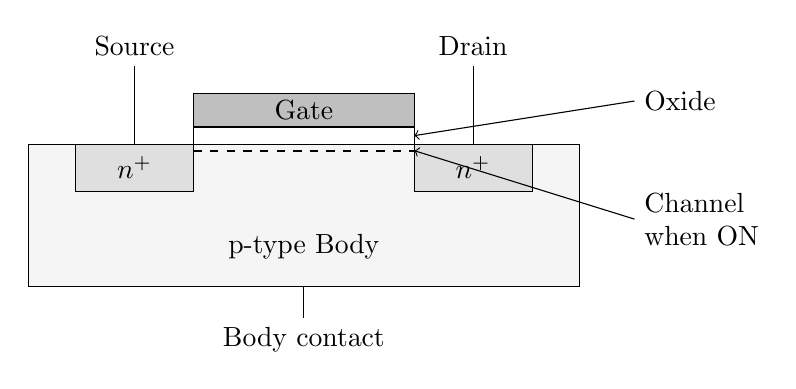
\begin{tikzpicture}[x=1cm,y=1cm]
\draw[fill=gray!8] (0,0) rectangle (7,1.8);
\draw[fill=gray!25] (0.6,1.2) rectangle (2.1,1.8);
\draw[fill=gray!25] (4.9,1.2) rectangle (6.4,1.8);
\node at (1.35,1.5) {$n^+$};\node at (5.65,1.5) {$n^+$};
\node at (3.5,0.5) {p-type Body};
\draw[fill=white] (2.1,1.8) rectangle (4.9,2.02);
\draw[fill=gray!50] (2.1,2.02) rectangle (4.9,2.45);
\node at (3.5,2.23) {Gate};
\draw (1.35,1.8)--(1.35,2.8) node[above] {Source};
\draw (5.65,1.8)--(5.65,2.8) node[above] {Drain};
\draw (3.5,0)--(3.5,-0.4) node[below] {Body contact};
\draw[<-] (4.9,1.91)--(7.7,2.35) node[right] {Oxide};
\draw[dashed,thick] (2.1,1.72)--(4.9,1.72);
\draw[<-] (4.9,1.72)--(7.7,0.85) node[right,align=left] {Channel\\when ON};
\end{tikzpicture}
\end{latin}
\caption{طرح آموزشی مقطع \lr{nMOS} بر پایه شکل \secnum{۱.۹} کتاب
\cite{weste}. خط‌چین محل تشکیل کانال را نشان می‌دهد؛ وجود همیشگی کانال را القا نمی‌کند.
خط اتصال بدنه فقط نمایش مفهومی پایانه است، نه طرح ساخت تماس.}
\label{fig:ch1-crosssection}
\end{figure}

در \lr{pMOS}، نوع ناحیه‌ها معکوس است: \lr{Source} و \lr{Drain} از نوع
\(p^+\) و بدنه از نوع \lr{n} هستند. در \lr{CMOS}، هر دو نوع روی یک تراشه
ساخته می‌شوند؛ به همین دلیل برای یکی از آن‌ها ناحیه مناسب \lr{Well} لازم است
\cite[صفحات چاپی ۷ و ۸]{weste}.
نام \lr{MOS} تاریخی است؛ جنس \lr{Gate} در دوره‌های مختلف یکسان نبوده است.

\subsection{تشکیل کانال در \lr{nMOS} و \lr{pMOS}}
برای \lr{nMOS} با بدنه و \lr{Source} نزدیک زمین، بالا بردن ولتاژ
\lr{Gate} الکترون‌ها را به سطح زیر عایق جذب می‌کند.
با ولتاژ کافی، نزدیک سطح کانالی با حامل غالب الکترون تشکیل می‌شود؛
این \lr{Inversion} مسیر هدایت میان دو ناحیه \(n^+\) را فراهم می‌کند
\cite[صفحه چاپی ۸]{weste}\cite[اسلایدهای ۶ و ۷]{mos}.
خاموش بودن یعنی مسیر کانال در مدل ساده برقرار نیست؛ این مدل جریان نشتی را حذف می‌کند.

در \lr{pMOS} با بدنه و \lr{Source} نزدیک تغذیه، پایین آوردن ولتاژ
\lr{Gate} نسبت به \lr{Source}، کانال حفره‌ای را ایجاد می‌کند.
بنابراین رفتار کنترلی آن مکمل \lr{nMOS} است.
این توصیف مقدماتی است؛ حالت‌های بار سطحی و روابط کمی در ابتدای فصل دوم استخراج می‌شوند.

\subsection{ولتاژ کنترل، آستانه و مدل \lr{Switch}}
برای \lr{nMOS} از اختلاف \(V_{gs}=V_g-V_s\) و آستانه مثبت \(V_{tn}\)
استفاده می‌کنیم. برای \lr{pMOS} در قرارداد اندازه‌های مثبت،
\(V_{sg}=V_s-V_g\) را با \(|V_{tp}|\) مقایسه می‌کنیم:
\begin{equation}\label{eq:ch1-threshold}
V_{gs}>V_{tn}\quad(\mathrm{nMOS}),\qquad
V_{sg}>|V_{tp}|\quad(\mathrm{pMOS}).
\end{equation}
در هر دو شرط، معیار اختلاف پتانسیل است، نه ولتاژ یک پایانه به‌تنهایی.
برابری با آستانه، مرز مدل ساده است؛ برای کاربرد عملی نمی‌توان آن را هدایت قوی دانست.
بدنه و آستانه نیز در مدل‌های دقیق‌تر مستقل از بایاس نیستند.

\textbf{مثال آموزشی.} در یک \lr{nMOS} فرضی با \(V_{tn}=\qty{0.3}{\volt}\)،
اگر \(V_g=\qty{1}{\volt}\) و \(V_s=\qty{0.9}{\volt}\)،
داریم \(V_{gs}=\qty{0.1}{\volt}\) و شرط روشن بودن برقرار نیست.
پس «\lr{Gate} بالا است» به‌تنهایی کافی نیست.
در گیت‌های ایستای متعارف که \lr{nMOS} خروجی را به زمین و \lr{pMOS} آن را
به تغذیه وصل می‌کند، ورودی‌های ریل‌به‌ریل این قاعده ساده را می‌دهند:
ورودی یک، \lr{nMOS} را روشن و \lr{pMOS} را خاموش می‌کند؛ ورودی صفر برعکس است
\cite[اسلاید ۲۱]{intro}. فرض می‌کنیم تغذیه از آستانه‌های لازم بیشتر است.

مدل \lr{Switch}، مسیر روشن را وصل و مسیر خاموش را قطع فرض می‌کند.
در آن، مقاومت مسیر، ظرفیت، نشتی و زمان روشن شدن را حذف می‌کنیم.
روشن بودن فقط امکان عبور جریان را نشان می‌دهد؛ بدون اختلاف ولتاژ یا بار مناسب،
جریان می‌تواند صفر باشد. شباهت تقریبی دو ناحیه \lr{Source} و \lr{Drain}
در شکل مقدماتی نیز مجوز نادیده گرفتن دیودهای بدنه یا محدودیت‌های یک قطعه واقعی نیست.

\subsection{پرسش کوتاه برای کنترل مدل}
\begin{enumerate}
\item \textbf{چرا \lr{Gate} عایق‌شده می‌تواند جریان کانال را کنترل کند؟}
کنترل با میدان الکتریکی و تغییر بار سطح انجام می‌شود؛ به عبور جریان اصلی از عایق نیاز ندارد.
\item \textbf{آیا بدون جریان رسانشی \lr{Gate}، ورودی هیچ انرژی نمی‌خواهد؟}
خیر؛ تغییر ولتاژ، ظرفیت ورودی را شارژ و دشارژ می‌کند.
\item \textbf{چرا بدنه را نباید حذف‌شده فرض کنیم؟}
پایانه چهارم بر پیوندها و آستانه اثر دارد؛ در این گام فقط اتصال متعارف و مدل ساده آن را به کار می‌بریم.
\end{enumerate}
